\chapter{Prétraitement des données}

\begin{Astuce}
Règle d'or du chapitre : \textbf{\og Garbage in, garbage out \fg{}} — des données sales
donnent des résultats faux. La préparation occupe \textbf{au moins 60\,\%} du temps d'un
projet (Dorian Pyle).
\end{Astuce}

\section{Pourquoi prétraiter ?}
Les données brutes sont souvent : \textbf{incomplètes} (valeurs manquantes),
\textbf{bruitées} (erreurs, exceptions), \textbf{incohérentes} (nommage, codage),
obsolètes ou mal formatées. Les 5 grandes étapes du prétraitement :
\textbf{Nettoyage} $\rightarrow$ \textbf{Intégration} $\rightarrow$ \textbf{Transformation}
$\rightarrow$ \textbf{Réduction} $\rightarrow$ \textbf{Discrétisation}.

\section{Données manquantes}
Causes : panne d'équipement, incohérence, non-saisie, oubli. Comment combler les
\og trous \fg{} ?
\begin{itemize}[leftmargin=1.4em]
  \item \textbf{Ignorer} l'enregistrement (peu efficace si beaucoup de manquants) ;
  \item \textbf{Remplir manuellement} (laborieux) ;
  \item \textbf{Constante globale} (\og inconnu \fg{}) ;
  \item \textbf{Moyenne} (variable numérique) ou \textbf{mode} (variable modale) ;
  \item \textbf{Moyenne par classe} (mieux) ;
  \item \textbf{Valeur la plus probable} (formule bayésienne / arbre de décision).
\end{itemize}

\begin{Calcul}[: combler un âge manquant de 3 façons]
Soit la colonne \texttt{Âge} $=[25,\ ?,\ 30,\ 40,\ 25]$ (une valeur manquante), avec une
classe associée $[\text{A},\text{A},\text{B},\text{B},\text{A}]$.
\begin{itemize}[nosep,leftmargin=1.4em]
  \item \textbf{Moyenne globale} : sur les 4 valeurs connues,
        $\overline{x}=\tfrac{25+30+40+25}{4}=30$ $\Rightarrow$ on met \textbf{30}.
  \item \textbf{Mode} (valeur la plus fréquente) : $25$ apparaît 2 fois $\Rightarrow$ on met \textbf{25}.
  \item \textbf{Moyenne par classe} : le manquant est de classe \og A \fg{} ; moyenne des âges
        de classe A connus $=\tfrac{25+25}{2}=25$ $\Rightarrow$ on met \textbf{25} (plus
        \og juste \fg{} car contextualisé).
\end{itemize}
\end{Calcul}

\section{Données bruitées}
\textbf{Bruit} = erreur ou variance aléatoire d'une variable mesurée. On le corrige par :
détection de points isolés, \textbf{clustering} (regrouper et repérer les isolés),
inspection humaine, ou \textbf{régression} (lisser par une fonction).

\section{Intégration \& redondance}
\textbf{Intégration} = combiner plusieurs sources en une seule. Problèmes : noms différents
pour la même donnée (\texttt{num\_client} $\equiv$ \texttt{client\_id}), unités différentes
(cm vs pouces). La \textbf{redondance} (un attribut déductible d'un autre) se détecte par
\textbf{analyse de corrélation}.

\section{Transformation des données}
Lissage, agrégation, généralisation, et surtout les deux mises à l'échelle au programme :

\begin{Definition}[Normalisation min-max]
Ramène chaque valeur dans l'intervalle $[0,1]$ :
\[ X^{*} = \frac{X - \min(X)}{\max(X) - \min(X)} \]
La plus petite valeur devient 0, la plus grande devient 1.
\end{Definition}

\begin{Definition}[Standardisation (z-score)]
Centre (moyenne 0) et réduit (écart-type 1) :
\[ X^{*} = \frac{X - \overline{X}}{\sigma(X)}, \qquad
   \overline{X}=\frac{1}{N}\sum_{i=1}^{N}x_i, \qquad
   \sigma^2=\frac{1}{N}\sum_{i=1}^{N}(x_i-\overline{X})^2 \]
Les valeurs tombent typiquement entre $-3$ et $+3$.
\end{Definition}

\begin{Calcul}[: min-max et z-score sur $X=\{200,150,300,100,250\}$]
\textbf{Min-max} : $\min=100$, $\max=300$, étendue $=200$.
\[ \frac{200-100}{200}=0.5;\quad \frac{150-100}{200}=0.25;\quad \frac{300-100}{200}=1;\quad
   \frac{100-100}{200}=0;\quad \frac{250-100}{200}=0.75 \]
$\Rightarrow X^{*}=\{0.5,\,0.25,\,1,\,0,\,0.75\}$ — bien dans $[0,1]$. \\[4pt]
\textbf{Z-score} — étape 1, la \emph{moyenne} :
$\overline{X}=\dfrac{200+150+300+100+250}{5}=\dfrac{1000}{5}=200$.\\
Étape 2, la \emph{variance} (moyenne des carrés des écarts à la moyenne) :
\[ \sigma^2=\tfrac{1}{5}\big[(200{-}200)^2+(150{-}200)^2+(300{-}200)^2+(100{-}200)^2+(250{-}200)^2\big]
   =\tfrac{0+2500+10000+10000+2500}{5}=5000, \]
donc l'écart-type $\sigma=\sqrt{5000}\approx 70{,}71$. Étape 3, on standardise chaque valeur :
\[ \frac{200-200}{70{,}71}=0;\ \frac{150-200}{70{,}71}=-0{,}71;\ \frac{300-200}{70{,}71}=+1{,}41;\
   \frac{100-200}{70{,}71}=-1{,}41;\ \frac{250-200}{70{,}71}=+0{,}71 \]
$\Rightarrow$ on vérifie : la nouvelle moyenne est $\approx 0$ et le nouvel écart-type $\approx 1$.
\end{Calcul}

\begin{figure}[ht]\centering
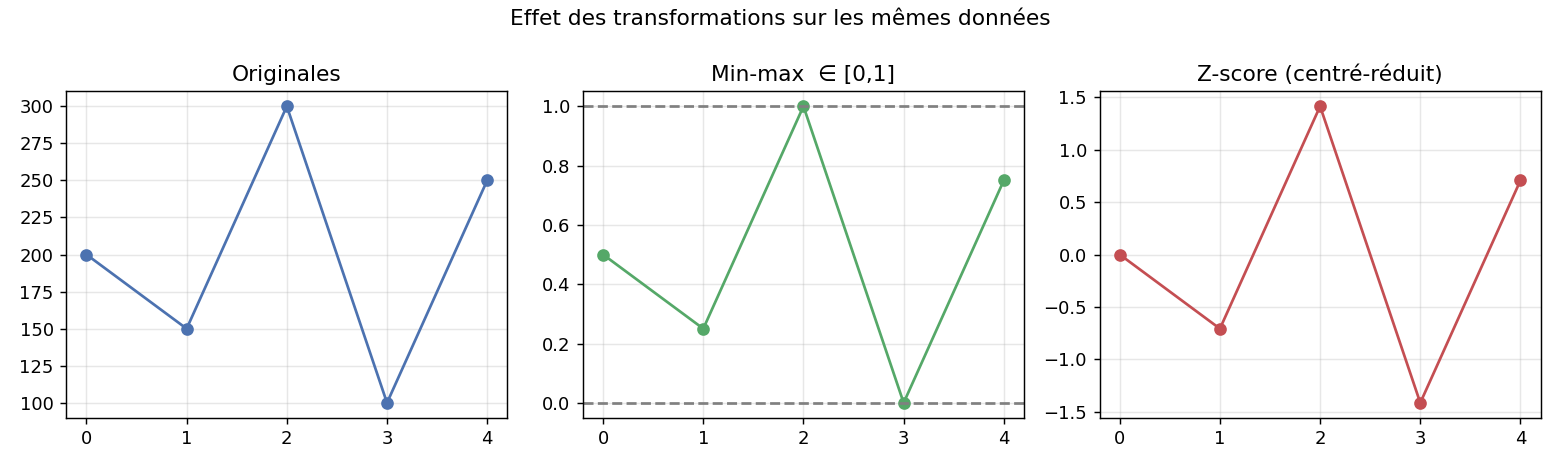
\includegraphics[width=0.95\linewidth]{figures/chap2_transformations.png}
\caption{Mêmes données vues en brut, après min-max (dans $[0,1]$) et après z-score (centré-réduit).}
\end{figure}

\section{Réduction des données}
Obtenir une représentation \textbf{plus petite} mais aux résultats \textbf{quasi identiques} :
agrégation par cubes, \textbf{réduction de dimension} (moins de colonnes/attributs),
réduction de numérosité (moins de lignes), discrétisation.

\section{Exercices résolus}

\subsection{Exercice 1 — repérer les problèmes de qualité}
\begin{center}\small
\begin{tabular}{cccccc}
\toprule
ID & Code postal & Sexe & Revenu & Âge & État civil\\
\midrule
1001 & 10048 & M & 75000 & C & M\\
1002 & J2S7K7 & F & -40000 & 40 & V\\
1003 & 90210 & \cellcolor{rougeclair}(vide) & \cellcolor{rougeclair}10000000 & 45 & C\\
1004 & \cellcolor{rougeclair}6269 & M & 50000 & \cellcolor{rougeclair}0 & C\\
1005 & 55101 & F & \cellcolor{rougeclair}999999 & 30 & D\\
\bottomrule
\end{tabular}
\end{center}

\begin{Calcul}[: problèmes détectés]
\begin{itemize}[leftmargin=1.4em,nosep]
  \item \textbf{Valeur manquante} : sexe absent (ligne 1003).
  \item \textbf{Valeur hors domaine} : revenu $=-40000$ (négatif, impossible).
  \item \textbf{Valeur aberrante} : revenu $=10\,000\,000$ (extrême).
  \item \textbf{Code de manquant déguisé} : revenu $=999999$ et âge $=0$ (faux \og vrais \fg{} chiffres).
  \item \textbf{Incohérence de type/format} : âge $=$ \og C \fg{} (non numérique) ;
        codes postaux mélangeant chiffres US (5 chiffres) et alphanumérique canadien (J2S7K7).
\end{itemize}
\end{Calcul}

\subsection{Exercice 2 — normalisation \& standardisation (dataset \texttt{churn})}
La démarche (que le script automatise) :
\begin{enumerate}[leftmargin=1.6em,nosep]
  \item vérifier les valeurs manquantes (\texttt{df.isna().sum()}) ;
  \item comparer \texttt{area code} et \texttt{state} (incohérences géographiques) ;
  \item transformer \texttt{day minutes} par \textbf{min-max} et vérifier sur une courbe que
        tout est dans $[0,1]$ ;
  \item transformer \texttt{night minutes} par \textbf{z-score} et lire l'intervalle obtenu
        (typiquement $[-3,+3]$).
\end{enumerate}

\section{Script Python commenté}
\lstinputlisting[caption={scripts/chap2\_normalisation.py — min-max, z-score, qualité},
  label=lst:chap2]{../scripts/chap2_normalisation.py}

\begin{Resume}
Prétraiter = nettoyer (manquants, bruit), intégrer (sources, redondance), transformer
(\textbf{min-max} dans $[0,1]$, \textbf{z-score} centré-réduit) et réduire. C'est l'étape la
plus chronophage mais elle conditionne tout le reste — en particulier le K-NN et le k-means
qui dépendent des distances.
\end{Resume}
